\documentclass[amsmath,amssymb,floatf
ix]{revtex4}
%\usepackage{graphicx}
\begin{document}
\preprint{APS/123-QED}
\title{Phase Transitions in Multiplicative Competitive Processes}
\author{Hideaki Shimazaki}
    %\email{hideaki@ton.scphys.kyoto-u.ac.jp}
    \affiliation{Department of Physics, Graduate School of Science, Kyoto University, Kyoto 606-8502, Japan}
\author{Ernst Niebur}
\affiliation{Department of Neuroscience, Zanvyl Krieger Mind/Brain
Institute, School of Medicine, Johns Hopkins University, Baltimore, Maryland
21218}
\date{\today}
\def\be{\begin{equation}}
\def\en{\end{equation}}
\newcommand{\figref}[1]{FIG.~\ref{#1}}
\newcommand{\Eq}[1]{Eq.~\ref{#1}}

\begin{abstract}
We introduce a discrete multiplicative process as a generic model of
competition. Players with different abilities successively join the
game and compete for finite resources.  Emergence of dominant players
and evolutionary development occur as a phase transition. The competitive dynamics underlying this transition is understood from a formal analogy to statistical mechanics.
The theory is applicable to bacterial competition, predicting novel population dynamics near
criticality.
\end{abstract}
\pacs{87.23.-n, 87.23.Kg, 05.45.-a, 03.75.Nt}
\maketitle

Competition occurs when two or more players such as organisms,
individuals or companies strive for common but limited resources. It
plays a significant role in biological and social activities, and is
the basis of evolution.
Most natural competition processes allow the
introduction of new players, which is a hallmark of an open,
nonequilibrium system.
In this contribution, we introduce an irreversible discrete multiplicative process with
normalization at each time step as a generic model of competition. Players with different abilities successively join the
game and compete for finite resources.  The model shows
macroscopically observable changes in its behavior; at a singularity
in the statistical distribution of the players' abilities, certain
players become dominant over all others.
The emergence of dominant
players and the evolutionary development of the system occur as a
transition from stationary to nonstationary state of the
multiplicative process.  We analyze the phase
transition in the mathematical framework of Bose-Einstein condensation
(BEC), although, of course, systems modelled are classical
and not quantum mechanical. The same approach has been applied
successfully to models of complex networks \cite{Bianconi01} and
ecosystems \cite{Volkov04} that behave
analogously to a Bose gas. We show that this approach is applicable to
bacterial competition, providing surprising insights and
predictions to their dynamics.

%\subsection*{Mean Field Approach to Multiplicative Competitions}
Before we present the model, we first introduce a general framework
for how our multiplicative competition model is related to a
statistical mechanics concept.
%a function $\varphi(\epsilon)$  is formally related to a Bose distribution.
Let $\varphi(\epsilon)$ be a function that satisfies the following
conditions for an arbitrary $C^2$ density function $g(\epsilon ) (\geq 0)$
defined on $\epsilon \in [0,\epsilon_{\max}]$,
\begin{eqnarray}
\int{d\epsilon \, g(\epsilon)} &=& 1, \label{33}\\
\int{d\epsilon \, g(\epsilon)\varphi (\epsilon)} &=& m + y_0, \label{34}\\
\int{d\epsilon \, g(\epsilon)e^{- \beta \epsilon} \varphi(\epsilon)} &=& M.
\label{35}
\end{eqnarray}
All terms on the right hand sides of these equations and $\beta$ in
\Eq{35} are positive constants. Then $\varphi(\epsilon)$ is given
by \be\label{36} \varphi(\epsilon) = \frac{y_0}{1 - e^{-\beta \epsilon
- \alpha}}, \en where $e^{-\alpha}=m/M$. For, dividing \Eq{34} by
$y_0$, then subtracting \Eq{33} yields \be\label{24} \int
{d\epsilon \, g(\epsilon)\frac{\varphi(\epsilon) - y_0}{y_0} } = N,
\en where $N = m/y_0$. Multiplying \Eq{35} with $ N/M$ and
subtracting \Eq{24} from the result,
the fundamental lemma of the calculus of variation then yields
\Eq{36}. Hence, the so-called occupation number in \Eq{24},
\be\label{37} n(\epsilon) = \frac{\varphi(\epsilon) - y_0}{y_0} =
\frac{1}{e^{\beta \epsilon + \alpha} - 1}, \en becomes the Bose
distribution. From \Eq{36}, such a function $\varphi(\epsilon)$ may
be obtained from the sum of a geometric progression with ratio
$e^{-\beta \epsilon - \alpha}<1$. This motivates the analysis of the
following multiplicative process.

The competition we introduce is defined by three conditions at each time
step.
(i) Players compete for a fixed total amount of resources.
(ii) The resource gained by a player is proportional to the player's innate
ability and to its resource gained at the previous time step.
(iii) New players join the game, each with the same initial resources. The
only exception is the first player (pioneer), who starts the game with all
the resources available.
These rules are summarized in a simple multiplicative process,
\be\label{1}
y_i(t+1) = a_i b(t)y_i(t),
\en
where $y_i(t)$ is the gain of the $i$th player at time $t$ and $a_i$ is its
ability, a positive and time-independent random variable chosen from a
distribution $\rho(a)$.
The term $b(t)$ is a normalization factor, which models the limited resources.
For simplicity, we first assume that $l$, the number of
newly introduced players at every time step, is 1. This means we consider $t
+ 1 $ simultaneous equations $(i=0, \cdots, t)$ at time $t$.
The normalization factor is then defined by $b(t) =
m/M_t$, where  $M_t$ is given by
\be\label{2}
M_t = \sum\limits_{j = 0}^t {a_j y_j (t)}.
\en
This assures that the amount of resources distributed among $t$ players at
time
$t$ is $m $ for $t > 0$.
The initial value of a new player is $y_i(i) = y_0$, except for the pioneer
whose initial value is $y_0(0)=m + y_0$. Therefore, the total resources
distributed among all players are limited to $m + y_0 $ at every time step.
Due to the normalization, we let $a \in [a_{\min},1]$, where $a_{\min}> 0$,
without loss of generality.

We now consider the time evolution of players except for the
pioneer. The gain of the $i$th player at time $t$ is given by
$y_i(t)=\Omega_i(t) y_0$, where
\be\label{3} \Omega _i(t) = a_i^{t-i}
\left( \prod\limits_{t'=i}^{t - 1}{b(t')} \right).  \en
The dynamics
given by $\Omega_i(t)$ shows distinct phases determined by the shape
of the ability distribution. To see this, we parameterize $\rho(a)$ by
the inverse temperature $\beta (=1/T) $ through $a = e^{ - \beta
\epsilon }$.
The random variable $\epsilon \in [0,\epsilon_{\max}]$ is chosen from $g(
\epsilon )$, a state density function which now defines the system.
We now systematically change $\rho(a) \left( = g(\epsilon)\left|
{{\textstyle{{d\epsilon } \over {da}}}} \right| \right)$ by fixing
$g(\epsilon)$ and changing $\beta$.  If $g(\epsilon)$ is a monotonically
increasing function, which we will assume, high
temperatures mean that the distribution of the players' abilities is
restricted to a small range, i.e. all players have relatively similar
abilities, while low temperature is synonymous with occasional
appearance of superior players relative to others.
From \Eq{3}, we have
\be\label{38} \ln \Omega_i = (t-i)\left\{-
\beta \epsilon_i - \left\langle {\ln b} \right\rangle \right\}, \en
using $\ln \prod\nolimits_{t'=i}^{t - 1} {b( t' )} = \sum\nolimits_{t'
= i}^{t - 1} {\ln b( t' )} \sim (t -i) \left\langle {\ln b}
\right\rangle$. By assuming stationarity of $M_t$, discussed below, we
let its time average be
\be\label{5}
\left\langle {\ln b} \right\rangle = -\alpha,
\en
where $\alpha$ is a time-independent
constant.  From \Eq{38} and \Eq{5}, we obtain $y_i(t) =
e^{(-\beta \epsilon_i - \alpha)(t-i)} y_0 $. Given $e^{-\beta
\epsilon_i - \alpha} < 1$, the cumulative gain $\varphi_t (\epsilon_i)
= \sum\nolimits_{t' = i}^t {y_i ( {t'} )} $, converges to $\varphi (
\epsilon_i )$ in \Eq{36}. Hence, the normalization of $\varphi _t
(\epsilon_i )$ by the initial value $y_0$,
%\be\label{10}
$n_t ( \epsilon_i  ) = \{\varphi_t (\epsilon_i) - y_0\}/{y_0}$,
approaches the Bose distribution in the thermodynamic limit $(t \to
\infty)$. Indeed, in this limit,
\be\label{11}
\mathop {\lim }\limits_{t \to \infty } M_t = \int {d\epsilon \,
g(\epsilon)\sum\limits_{t'=0}^\infty {e^{- \beta \epsilon} y(t')} },
\en
%where $y(t') = e^{(-\beta \epsilon  - \alpha)t'}y_0$.
where $\sum\nolimits_{t'=0}^\infty y(t') = \varphi(\epsilon)$.
As the assumption of stationarity yields $\mathop {\lim }\limits_{t \to
\infty } \ln b( t ) = \left\langle {\ln b} \right\rangle $, we have $\mathop
{\lim }\limits_{t \to \infty } {m \mathord{\left/ \right.} {M_t }} = e^{ -
\alpha } $ from \Eq{5}.
%Substituting this into \Eq{11} yields% an
%equality,
By substituting this into \Eq{11}, we obtain a self-consistent
equation,%an equality,
\be\label{13}
\int {d\epsilon \, g(\epsilon)\frac{1}{e^{\beta \epsilon + \alpha } - 1}} =
N,
\en
where $N = m/y_0$.  Note that we can generalize  \Eq{1} such that we
allow $l (\geq 1)$ new players to join the competition with initial
value $y_0$ at each step. From a similar argument, we obtain
\Eq{13}, where $N = m / y_0 l$.  Thus the deduced form \Eq{13}
of the competition under stationarity assumption shows a formal analogy to
those obtained for a quantum gas. The
normalization factor $\alpha$ plays the role of keeping
the total resources gained by all players constant at every time step;
in analogy to the chemical potential of a quantum gas which is introduced for the conservation of particle number. According to this reasoning, condensation of resources to a single player analogous to BEC is expected at low temperature where
$\alpha$ vanishes.


%\subsection*{Emergence of Dominance and Evolution}
To study this prediction, we simulate the multiplicative process
\Eq{1}, adopting a standard density function, \be\label{39}
g(\epsilon) = C_\sigma \epsilon^{\sigma-1}, \en where $C_\sigma =
\sigma / \epsilon_{\max}^\sigma$ $(\sigma>1)$. We find two distinct
phases for the distribution of the normalized cumulative gain
$n_t(\epsilon_i) = \{\varphi_t (\epsilon_i) - y_0\}/{y_0}$. At high
$T$, $n_t(\epsilon_i)$ obeys the Bose distribution
(\figref{PT}-a). At low $T$, the coordinated distribution breaks
down: players with low energy (high ability) dominate a large fraction
of the cumulative gain.  This condensate exists only below a
critical point $\alpha=0$. For, if $\alpha $ is negative, $\varphi (
\epsilon_i )$ of the player with $\epsilon_i < -\alpha / \beta$ does
not converge. Its normalized cumulative gain can not be incorporated
in the integral in \Eq{13}; rather it has to be added as an extra
term.  The critical temperature for this transition can be predicted
in the usual way: Change of variables $y = \beta \epsilon $ and use of
$\alpha=0$ in \Eq{13} yields
\be\label{15} N = \frac{\sigma
}{(\beta \epsilon_{\max})^\sigma} \int_0^{\beta \epsilon _{\max} }
{\frac{{y^{\sigma - 1} }}{e^y - 1} \,dy}.  \en
By approximating the
upper limit of integral in \Eq{15} by infinity, the critical
temperature $T_c({ = 1/\beta _c })$ is given by
\be\label{17} T_c^{( 1
)} \sim \epsilon _{\max} \left\{ {N^{ - 1} \Gamma(\sigma + 1)
\zeta(\sigma)} \right\}^{ - {\textstyle{\frac{1}{\sigma} }}}, \en
for $N \ll 1$. When $N \gg 1$, this approximation is not valid because of
the high critical temperature; instead, from   $e^y \simeq 1 +
y$ and \Eq{15},  one obtains
\be\label{32} T_c^{(2)} \sim
\epsilon_{\max}(1 - \sigma^{-1}) N.  \en
The transition can be seen in
the occupation by the most capable player, defined by ${\varphi_t
(\epsilon_{\min})} \mathord{\left/ {\sum\nolimits_j {\varphi_t (
{\epsilon_j } )} } \right.} $. As $T$ decreases below $T_c$, its
occupation dramatically increases, supporting the prediction
(\figref{PT}-c).

%FIG1 HERE
\begin{figure}[t]
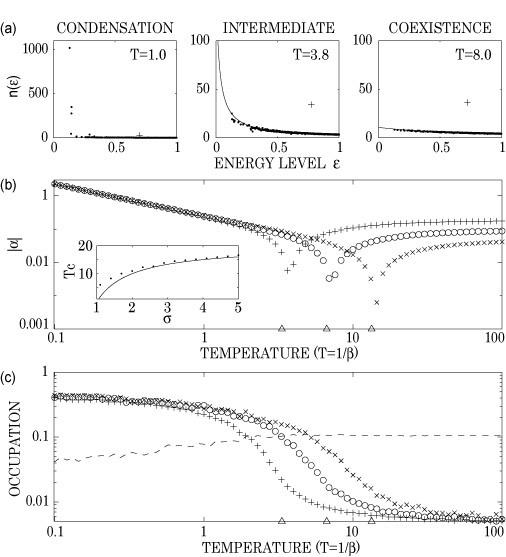
\includegraphics[width=8.7cm]{FIG1}
\caption{\label{PT}
(a) Normalized cumulative gain $n_t(\epsilon_i)$
%\Eq{10}
for $m = 5$ and $T<T_c$ (left), $T \approx T_c$ (center) and $T>T_c$
(right). Solid line is the Bose distribution with $\alpha $ from
\Eq{5}. Plus sign indicates a pioneer. Plots of the last ten
entrants were excluded. (b) Numerical calculation of $|\alpha|$ with
$\alpha$ from \Eq{5}, averaged over 500~trials. Symbols +, o, x
indicate $m = 5$, $10$ and $20$.  Change in the sign of $\alpha$
indicates the transition. Triangles on the abscissa are the transition
temperatures from \Eq{32}; $T_c \approx 3.33 $, $6.67 $ and $13.3
$. Shown in inset is the dependence of $T_c$ on exponent $\sigma $ for
$m = 20$ (dots) and the analytical solution from \Eq{32}, solid
line. (c) Cumulative occupation by the most capable player was
calculated from $ \varphi_t (\epsilon _{\min}) / \sum\nolimits_j
\varphi_t (\epsilon _j) $ at
%$\epsilon_{\min} = \min \left\{ \epsilon_j \right\} $ and
$t = 200$. Symbols as in (b). Dashed line, occupation by pioneer for $m =
20$. In all simulations, $y_0 = 1 $, $l = 1$, $\sigma = 3$ and $\epsilon
_{\max } = 1$.}
\end{figure}

We verified the existence of a BEC analogue in a discrete
multiplicative process, as was shown in a continuous model
\cite{Bianconi01}. However, we emphasize that, as a matter of
principle, our classical dynamical system is not equivalent to a
quantum gas. The most important difference is based on the following
observation. The time evolution of each player's gain
is different above and below the predicted $T_c$. Above $T_c$, the
gains of all players monotonically decrease.
Below $T_c$, not all of them show monotonic behavior, and the
competitive dynamics is disordered.  The
observed nonequilibrium phase transition from ordered to disordered
state occurs as a violation of the stationarity in weighted mean
ability, $M_t/(m+y_0)$.  It is stationary if the
gain of all players monotonically decreases to zero, which allows the
argument below \Eq{38}. Otherwise, if the gain of one player rises
to dominate the resources, the weighted mean ability approaches the
ability of this one dominant player.  Then due to the replacement of
the dominant player upon the entrance of a player with higher ability,
we observe an irreversible increase of the weighted mean ability,
indicating that the system is now \textit{evolving}. Thus dominance
and evolution are aspects of nonstationary dynamics. We emphasize that
the phase transition yielding evolution does not happen in
equilibrium systems.

%\subsection*{Application to Biological Competition}
We now consider application of the theory to competition of clonal strains of asexual
\textit{Escherichia coli} serially propagated on glucose-limited medium. The population dynamics is most suitably described by a stochastic branching process with
mutation and selection. Consider the $i$th strain with
fitness $a_i$, mutation rate $\eta$, and population size
$y_i(t)$.
Let $y_i(t+1)$ ($i = 1, \cdots, Q(t)$) be given by
a Poisson distribution with mean
%\begin{equation}\label{21}
$  \lambda_i = \tilde{m} \frac { (1-\eta) a_i y_i(t) }{\sum_{i=0}^{Q(t)}
{ a_i y_i(t)} }.$
%\end{equation}
Here $Q(t)$ is the number of mutants that were
generated and that survived the initial step since the process
started.
%$Q(t)$ is also determined by a stochastic process.
The number of mutants produced at time $t$, $Q(t+1)-Q(t)$, is drawn from a
Poisson distribution with mean
%\begin{equation}\label{22}
$ l = \tilde{m} \frac { \sum_{j=0}^{Q(t)} {\eta a_j y_j(t)} } {
\sum_{i=0}^{Q(t)} { a_i y_i(t)} }$.
%\end{equation}
Note that the average total number of cells at time $t$ is fixed to
$\sum_{i=0}^{Q(t)} \lambda_i + l = \tilde{m}$ due to the normalization
factor in the above equations.

It is clear that our process \Eq{1} is a deterministic approximation
of this stochastic population dynamics. A monotonically decreasing
fitness distribution $\rho(a)$ should be used because most mutations
are likely to be deleterious \cite{Fisher58}.  We thus decided to use
the same $\rho(a)$ used in the analysis of the deterministic model (and
the state density \Eq{39}) because it satisfies this basic tenet.  Our
results do not depend, however, on the precise form of the state
density; other parameterizations of the fitness distribution of
$\rho(a)$ such as the beta distribution defined on $ a \in [0,1]$
yield essentially the same results (not shown).

\textit{Routes to Adaptive Evolution:}
A strong prediction of the theory is the existence of a singular point
on the emergence of evolution. We observed the transition from
stationary to non-stationary state in the numerical simulation of the
stochastic process by decreasing the temperature $T$. The
transition point is predictable from the critical temperature $T_c$
obtained by the deterministic theory (\Eq{32}). Above $T_c$, dominance
by a capable player (strain) appears. Below $T_c$, the dynamics are
governed by the random drift of dominant strains. The random fluctuation of dominant
strains is the most striking difference from dynamics of the deterministic model.

Another route to generate an
evolutionary development is to increase $T_c$ by fixing $T$.  The
critical temperature given by \Eq{32} is proportional to $N$, which is related to
mutation rate through $\eta = {l} /(m + l) = (N + 1)^{-1}$.
We thus obtain
\be \label{23} T_c \sim \epsilon_{\max}(1-\sigma^{-1}) ( \eta^{-1} - 1). \en
Given $T$, decreasing $\eta$ increases $T_c$ such that $T<T_c$ is
achieved. A sufficiently low mutation rate not only prevents
deleterious offspring but is necessary for adaptive evolution itself.
The deleterious role of high mutation rate to adaptive evolution termed as
`clonal interference' was observed in experiments of \emph{E. coli}
competition \cite{deVisser99}, and theoretically investigated elsewhere
\cite{Gerrish98}.

%FIG2 HERE
\begin{figure}[t]
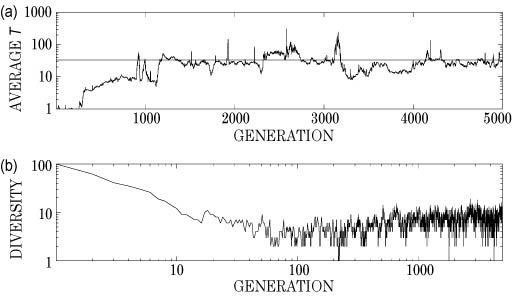
\includegraphics[width=8.7cm]{FIG2}
\caption{\label{SOC}
A stochastic branching process with mutation and selection described
in the text approaches a critical state by natural selection. Average total population is $\tilde{m}=100$. Simulation started with $100$ unique strains whose fitness is drawn from a fitness distribution with $T=1$, $\sigma = 3/2$ and $\epsilon_{\max}=1$. The $i$th strain produces mutants (mutation rate $\eta = 0.01$) whose fitness is drawn from a fitness distribution with $T_i$ given by \Eq{40} ($\gamma = 2$). (a) Average temperature of the system stays near the transition point $T_c = 33$. In early stages, the average temperature increases, indicating initial adaptive evolution.
(b) Number of existing strains at each steps (Diversity) decreases during initial adaptive evolution. However, further dominance by a few species is suppressed as the system approaches near criticality.
}
\end{figure}
\textit{Approach to the Transition Point by Natural Selection:}
An important question is wether $T$ is comparable to
$T_c$ under natural conditions.
Evolutionary progress observed in laboratory
experiments of \emph{E. coli} competition shows alteration of
long periods of relative stasis with short bursts of rapid change caused by
rare beneficial mutations \cite{Elena96}.
Therefore, empirically observed
dynamics is consistent with model behavior at $T < T_c$ in our construct at least during early stages of competition.
However, we argue that there exists a biologically plausible scenario in which
$T$ may eventually become comparable to $T_c$ by internally tuning
the parameter \cite{Bak87,Kauffman91}.

Instead of using a common fitness distribution for all strains, it
is physiologically plausible to assume that each strain has its
unique fitness distribution. We assume that fitness of mutants originating
from the $i$th strain of fitness $a_i$ is drawn from a fitness distribution
characterized by the temperature $T_i = 1/\beta_i$.
Since most mutants are deleterious, the average fitness
produced with $\beta_i$ should be less than $a_i$ (i.e. $\left\langle
a \right\rangle = e^{ - \beta_i \left\langle \varepsilon
\right\rangle }< a_i$, where $\left\langle \varepsilon \right\rangle
= \varepsilon _{\max } {\sigma \mathord{\left/ {\vphantom {\sigma
{\left( {\sigma + 1} \right)}}} \right.  \kern-\nulldelimiterspace}
{\left( {\sigma + 1} \right)}}$ for the state density
\Eq{39}.). Henceforth, the inverse temperature $\beta_i$ is given by
\be\label{40} \beta _i = - \gamma \left\langle \varepsilon
\right\rangle ^{ - 1} \ln a_i, \en where $\gamma > 1$ to satisfy
$\left\langle a \right\rangle < a_i$.

At the beginning of adaptive evolution, strains with higher fitness are
chosen by natural selection. Dominance by strains with high fitness
increases the average temperature of the population. Suppose that
adaptive evolution achieves a neutral condition, $T>T_c$. It is then by
chance wether or not a certain strain is picked up. Since a dominant
strain is prone to produce mutants inferior to the dominant strain
itself, those deleterious strains are likely to be picked up, and the
average temperature decreases.
There are ever going cycles of adaptive evolution, neutral state then collapse of the dominance (\figref{SOC}).
The advantage of the dynamics that approaches
criticality is rather clear. It allows initial adaptive evolution,
permanently eliminating unfavorable genotypes, but then significantly
slowing down or preventing further evolution
and dominance: close to the  critical state,
strains can co-exist for a substantial period of time.
Diversity introduced by the dynamics near criticality is clearly advantageous for the whole
ecosystem, which is exposed to global environmental changes. We thus conjecture that this strategy might be taken by some haploid species.

%\subsection*{Acknowledgement}
We thank H.G. Schuster and S. Shinomoto for very helpful
comments. Supported by the Murata Overseas Scholarship Foundation (HS)
and NIH grant R01 NS43188-01A1 (EN).

\bibliography{bec}


\end{document}



